\section{Choosing an Operating System}
        A raspberry pi is a small portable sized computer that has an ability to
        do powerful processing i.e. run applications etc. Just as any other computer
        it requires an OS to function. The device supports different
        types of operating systems like raspbian, Linux, Android things etc. I would like to 
        make a comparison between raspbian and android things in detail 
        and determine which OS fits best for our use case.

        \subsection{Raspbian}
            Raspbian is a free operating system, which is debian based specially optimized 
            for the Raspberry pi \cite{raspbien}. This is one of the most popular OS for
            the Raspberry pi hardware. 

        \subsection{Android Things}
            Android Things is a relatively new Operating system in the \textbf{IoT} 
            \cite{IoT} world. The operating system is developed by google, 
            which provides a new android framework APIs and allows you 
            to create rapid prototypes \cite{androidThings}. Figure 
            \ref{fig:aThingsOverview} gives an overview on the different 
            abstraction layers of Android Things. 
            \begin{figure}[htbp!]
                \centering 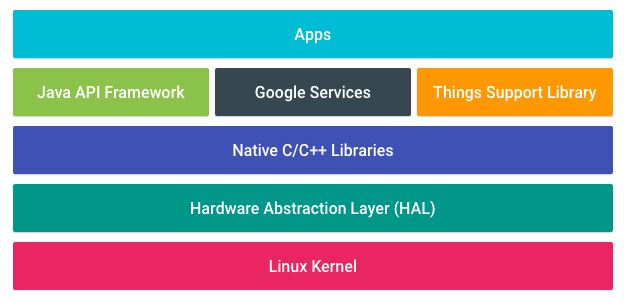
\includegraphics{grafiken/androidThingsOverview.jpg}
                \caption{Android Things OS Overview}
                \label{fig:aThingsOverview}
            \end{figure}
    
        
        \newpage
        \subsection{Comparison and Conclusion} 
            \label{ssec:OsComparison}  
            \begin{table}[h!]
                \centering
                \begin{tabular}{|p{9cm}|p{7.5cm}|}
                    \hline
                        \textbf{Android Things}  & \textbf{Raspbian}\\
                    \hline
                        Fast prototyping can be done because of the simplicity of setting
                        up a new project 
                        \url{https://developer.android.com/training/basics/firstapp/index.html}. & 
                        More development boards i.e. rpi2, raspberry pi zero etc. are supported\\
                    \hline
                        The existing android development tools, APIs and the huge resource library 
                        can be leveraged for easy development.
                        & It is more flexible in terms of what can be done since
                        it is an open-source OS.\\
                    \hline
                        It has very easy to use API's to connect to the development hardware.
                        \url{https://developer.android.com/things/sdk/pio/index.html} & Great
                        community support since there are more users.\\
                    \hline
                        Managing dependencies is very easy because the android development 
                        architecture is being used. It uses gradle to maintain the dependencies.
                        \url{https://gradle.org/}. & The OS is optimized for efficient use for
                        raspberry pi hardware.\\  
                    \hline
                \end{tabular}
                \caption{Comparision between Android Things and Raspbian}
                \label{table:aThingsVsRaspbian}     
        \end{table}

        \newpage 
        \par
            Both the operating systems have their own advantages and it would be biased to state that
            one of them is better than the other. After careful consideration and research, I
            decided to design the navigation module with Android Things which use Java as its
            programming language. The reasons why I choose android over raspbian are as follows:
            \begin{enumerate}
                \item 
                    Good and easy to understand documentation of how to setup 
                    a new project.
                \item 
                    Familiarity with the android and Java environment which increased my
                    productivity level.  
                \item 
                    The app written for the raspberry pi is similar to how one would
                    do it for native android so porting the app later to a native android
                    app if wanted would not be an issue. 
                \item 
                    The Java programming language has been around for a long time and many
                    frameworks to implement the software design patterns are readily 
                    available.
                \item 
                    The android environment makes it easy to handle dependencies using gradle
                    dependency manager, which is universal to all android packages. So the 
                    dependencies managing is not a issue if someone new installs the project.  
                \item
                    It has sample code examples for available APIs in github 
                    \url{https://developer.android.com/things/sdk/samples.html}. 
                \item
                    Android has a lot of frameworks which makes it easier to interface with an
                    external server via HTTP request \cite{http}.
            \end{enumerate}